\section{Experiment
	\label{ableitung:section:resultate}}
\rhead{Resultate}
Die Resultate dieser Arbeit sollen hauptsächlich zeigen, ob die
Finite Differenzen Methode als Option zur Optimierung neuronaler
Netzwerke geeignet ist.
Es ist klar, dass implementationsbedingt die Trainingsgeschwindigkeit dem Backpropagation-Algorithmus nicht das Wasser reichen kann.
Viel wichtiger ist eine qualitative Aussage machen zu können, ob die Methode eine interessante Variante darstellt und ob das Gedankenexperiment funktioniert.

Um dies an einem einfachen Beispiel zu verdeutlichen, wird versucht,
eine logische XOR-Verknüpfung zu trainieren.
Ein XOR-Gate ist ein elektronisches Bauteil, welches eine
{\em Entweder-Oder}-Logik abbildet.
\index{XOR}%
Im gewählten Fall hat das Bauteil zwei digitale Eingänge.
Ist entweder der Erste oder der Zweite aktiv, so ist der Ausgang
ebenfalls aktiv.
Ist keiner der beiden Ausänge oder beide Ausgänge aktiv,
so ist der Ausgang inaktiv.
Dies kann man der Logiktabelle in Abbildung \ref{ableitung:fig:xor-gate-logic} entnehmen.
\index{Logiktabelle}%
\begin{figure}[h]
	 \centering
	\begin{tikzpicture}
	
	\node (y) at (3, 1) {$y_1$};
	
	\node[american xor port, draw, number inputs=2] at (1.5, 1) (notx) {};
	
	\draw (notx.in 1 -| -1,0) -- (notx.in 1);
	\draw (notx.in 2 -| -1,0) -- (notx.in 2);

	\node at (notx.in 1 -| -1,0) [left] {$x_1$};
	\node at (notx.in 2 -| -1,0) [left] {$x_2$};

	\draw (notx.out) -- (y);
	
	\node at (7,1) {
	\begin{tabular}{cc|c}
		\hline
		$x_1$ & $x_2$ & $y$ \\
		\hline
		0 & 0 & 0 \\ 
		0 & 1 & 1 \\ 
		1 & 0 & 1 \\ 
		1 & 1 & 0 \\
		\hline						
	\end{tabular}};
	\end{tikzpicture}	
	\caption{Das XOR-Gate und die dazugehörige Logiktabelle}
	\label{ableitung:fig:xor-gate-logic}
\end{figure}
\tikzstyle{inputNode}=[draw,circle,minimum size=17pt,inner sep=0pt]
\tikzstyle{stateTransition}=[-stealth, thick]
\begin{figure}
	\centering
	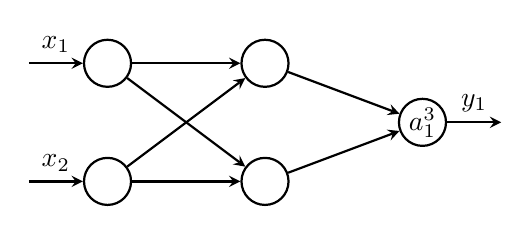
\begin{tikzpicture}
	
	\node[inputNode, thick] (i1) at (5, 1.5) {};
	\node[inputNode, thick] (i2) at (5, 0) {};
	
	\node[inputNode, thick] (h1) at (7, 1.5) {};
	\node[inputNode, thick] (h2) at (7, 0) {};
	
	\node[inputNode, thick] (o1) at (9, 0.75) {$a^{3}_{1}$};
	
	\draw[stateTransition] (4, 1.5) -- node[above] {$x_1$} (i1);
	\draw[stateTransition] (4, 0) -- node[above] {$x_2$} (i2);
	
	
	\draw[stateTransition] (i1) -- (h1);
	\draw[stateTransition] (i1) -- (h2);
	\draw[stateTransition] (i2) -- (h1);
	\draw[stateTransition] (i2) -- (h2);
	
	\draw[stateTransition] (h1) -- (o1);
	\draw[stateTransition] (h2) -- (o1);
	
	\draw[stateTransition] (o1) -- node[above] {$y_1$} (10, 0.75);

	\end{tikzpicture}
	\caption{Das neuronale Netzwerk zum Erlernen des XOR Logikoperators}
	\label{ableitung:fig:nn-result-net}
\end{figure}
Das gewählte Netzwerk, um diese Logik abzubilden, besteht aus drei
Schichten und ist in Abbildung \ref{ableitung:fig:nn-result-net}
ersichtlich.
Die Mittelschicht (hidden layer) wird benötigt, da sich mit nur
\index{hidden layer}%
\index{Mittelschicht}%
einer Schicht keine Lösung finden lässt, welche die zwei Inputs auf den Output abbilden kann.
In Abbildung \ref{ableitung:fig:visualisation-surface} wird das Ganze im zweidimensionalen Raum visualisiert.
Um die Kriterien der Logiktabelle umsetzten zu können, wird eine Sattelfläche im dreidimensionalen Raum benötigt. Eine Lösung ist in Abbildung \ref{ableitung:fig:visualisation-surface-2} ersichtlich, welche diese Anforderungen erfüllt.
\begin{figure}
	\centering
		%\documentclass[margin=10pt]{standalone}
%\usepackage{pgfplots}
\pgfplotsset{compat=1.13}% <- immer compat setzen!
\usepgfplotslibrary{fillbetween}
%\begin{document}
	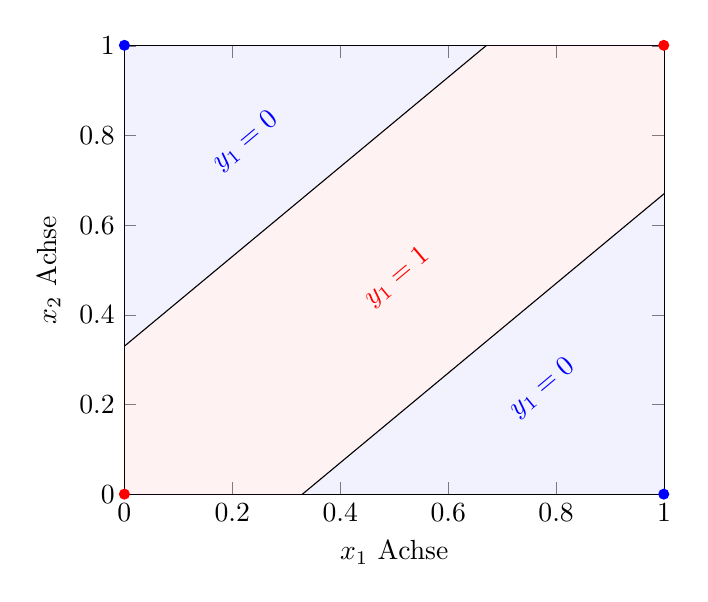
\begin{tikzpicture} 
	\begin{axis}[
	domain=0:1,% geändert
	xmin=0, xmax=1,
	ymin=0, ymax=1,
	xlabel = $x_1$ Achse,
	ylabel = $x_2$ Achse
	]

	\path[name path=axisy] (0,1) -- (1,1);
	\path[name path=axisx] (0,0) -- (1,0);



	\addplot+[mark=none, color=black, name path=A] {\x+0.33}
		node[above, color= blue, rotate=40] at (0.8,0.2) {$y_1=0$}
		node[above, color= blue, rotate=40] at (0.25,0.75) {$y_1=0$}
	;
	\addplot+[mark=none, color=black, name path=B] {\x-0.33} 
		node[below, color=red, rotate=40] at (0.48,0.52) {$y_1=1$}
	;
	
	\addplot [blue,fill opacity=0.05]
	fill between[of=A and axisy]
	;
	\addplot [blue,fill opacity=0.05]
	fill between[of=B and axisx]
	;
	
	\addplot [red,fill opacity=0.05]
		fill between[of=A and B]
	;
	    

	\end{axis} 
	
	\coordinate (a) at (0,0);
	\fill[red] (a) circle (2pt);
	\coordinate (b) at (6.85,5.7);
	\fill[red] (b) circle (2pt);
	
	\coordinate (c) at (0,5.7);
	\fill[blue] (c) circle (2pt);
	\coordinate (d) at (6.85,0);
	\fill[blue] (d) circle (2pt);
	
	\end{tikzpicture}
%\end{document}
		\caption{Visualisierung der Punkte in der $x_1$-$x_2$-Ebene und deren
		Separierbarkeit.}
	\label{ableitung:fig:visualisation-surface}
\end{figure}
\begin{figure}
	\centering
	%\documentclass{article}
%\usepackage{tikz}
%\usepackage{pgfplots}
%\pgfplotsset{compat=1.13}
%\begin{document}
  \begin{tikzpicture}
    \begin{axis}[
	    xmin=0, xmax=1,
	    ymin=0, ymax=1,
	    zmin=0, zmax=1,
	    xlabel={$x_1$},
	    ylabel={$x_2$},
	    zlabel={$y_1$},
	    view={30}{35}, grid=both]
	 \addplot3 [surf, mesh/rows=11, mesh/cols=11]
	    table[x=x, y=y, z=out, col sep=comma] {papers/ableitung/data/xor_raw_data.csv};
    \end{axis}
  \end{tikzpicture}
%\end{document}
	\caption{Visualisierung der Sattelfläche für den Output $y_1$.}
	\label{ableitung:fig:visualisation-surface-2}
\end{figure}
Das Experiment wurde basierend auf dem PyTorch Framework implementiert.
\index{PyTorch Framework}%
Das Netzwerk wurde jeweils mit der Finiten Differenzen Methode und dem Backpropagation-Algorithmus trainiert.
Bei der FDM wurden verschiedene Anzahlen an Stützstellen (Support) gewählt und unterschiedliche Abstände $h$ verwendet.
Die Resultate sind in den Abbildungen \ref{ableitung:fig:xor_h1},
\ref{ableitung:fig:xor_h01}, \ref{ableitung:fig:xor_h1} zusammengestellt.
Die vertikale-Achse in den Abbildungen stellt den quadratischen Fehler zwischen $\hat{y}$ und $y$ dar, während die horizontale-Achse die Entwicklung über die Anzahl Iterationen aufzeigt.

\begin{figure}
	\begin{tikzpicture}
	\begin{semilogyaxis}[xmin=0, xmax=1000, ymin=10e-15, ymax=10, width=\textwidth, height=0.30\textheight]
	\addplot[one, line width=1pt] table [x=epoch, mark=none, y=loss, col sep=comma] {papers/ableitung/data/backprop.csv};
	\addplot[two] table [x=epoch, mark=none, y=loss, col sep=comma] {papers/ableitung/data/h1-support2.csv};
	\addplot[three] table [x=epoch, mark=none, y=loss, col sep=comma] {papers/ableitung/data/h1-support4.csv};
	\addplot[four] table [x=epoch, mark=none, y=loss, col sep=comma] {papers/ableitung/data/h1-support6.csv};
	\addplot[five] table [x=epoch, mark=none, y=loss, col sep=comma] {papers/ableitung/data/h1-support8.csv};
	
	\addlegendentry{Backprop}	
	\addlegendentry{Support: 2}
	\addlegendentry{Support: 4}
	\addlegendentry{Support: 6}
	\addlegendentry{Support: 8}
	
	
	\end{semilogyaxis}
	\end{tikzpicture}
	\caption{Resultate des Gradientenabstiegs mit Stützstellenabstand $h=1$.}
	\label{ableitung:fig:xor_h1}
\end{figure}

\begin{figure}	
	\begin{tikzpicture}
	\begin{semilogyaxis}[xmin=0, xmax=1000, ymin=10e-15, ymax=10, width=\textwidth, height=0.3\textheight]
	\addplot[one, line width=1pt] table [x=epoch, mark=none, y=loss, col sep=comma] {papers/ableitung/data/backprop.csv};
	\addplot[two] table [x=epoch, mark=none, y=loss, col sep=comma] {papers/ableitung/data/h01-support2.csv};
	\addplot[three] table [x=epoch, mark=none, y=loss, col sep=comma] {papers/ableitung/data/h01-support4.csv};
	\addplot[four] table [x=epoch, mark=none, y=loss, col sep=comma] {papers/ableitung/data/h01-support6.csv};
	\addplot[five] table [x=epoch, mark=none, y=loss, col sep=comma] {papers/ableitung/data/h01-support8.csv};
	
	\addlegendentry{Backprop}	
	\addlegendentry{Support: 2}
	\addlegendentry{Support: 4}
	\addlegendentry{Support: 6}
	\addlegendentry{Support: 8}
	
	
	\end{semilogyaxis}
	\end{tikzpicture}
	\caption{Resultate des Gradientenabstiegs mit Stützstellenabstand $h=0.1$.}
	\label{ableitung:fig:xor_h01}
\end{figure}
	
\begin{figure}
	\begin{tikzpicture}
	\begin{semilogyaxis}[xmin=0, xmax=1000, ymin=10e-15, ymax=10, width=\textwidth, height=0.3\textheight]
	\addplot[one, line width=1pt] table [x=epoch, mark=none, y=loss, col sep=comma] {papers/ableitung/data/backprop.csv};
	\addplot[two] table [x=epoch, mark=none, y=loss, col sep=comma] {papers/ableitung/data/h001-support2.csv};
	\addplot[three] table [x=epoch, mark=none, y=loss, col sep=comma] {papers/ableitung/data/h001-support4.csv};
	\addplot[four] table [x=epoch, mark=none, y=loss, col sep=comma] {papers/ableitung/data/h001-support6.csv};
	\addplot[five] table [x=epoch, mark=none, y=loss, col sep=comma] {papers/ableitung/data/h001-support8.csv};
	
	\addlegendentry{Backprop}	
	\addlegendentry{Support: 2}
	\addlegendentry{Support: 4}
	\addlegendentry{Support: 6}
	\addlegendentry{Support: 8}
	
	
	\end{semilogyaxis}
	\end{tikzpicture}
	\caption{Resultate des Gradientenabstiegs mit Stützstellenabstand $h=0.01$.}
		\label{ableitung:fig:xor_h001}
\end{figure}

Es ist erstaunlich, dass bereits bei diesem kleinen Netzwerk numerische Effekte im Backpropagation-Algorithmus in einem etwas höheren Fehler resultieren.
Der Fehler von $\approx 10^{-14}$ im besten Fall (FDM) ist um Faktor
$10^3$ kleiner als die des Backpropagation-Algorithmus.
	
